
\chapter{Black-box TFNP} \label{chap:bb-tfnp}

\section{Oracles and decision trees}

In the previous chapter, we have briefly shown how \TFNP subclasses are defined in terms of basic existence principles that capture white-box total search problems solvable by protocols reducible to Karchmer-Widgerson games. From now on, we will shift our focus to the black-box model.

Black boxes have been used by complexity theorists since the early days, mostly through the concept of \textbf{oracle}, a device capable of instantly solving an instance of a designated problem. In particular, these problems may even be uncomputable, an assumption that allows us to view oracles as magical devices. Turing machines can be allowed to query such oracles to an additional \textit{oracle tape}. The machine writes a string on such tape, asking the oracle to solve the problem for that input. The output of the oracle is then written on the same tape, which can then be read by the Turing machine. Any query made to the oracle requires $\Theta(1)$ time, meaning that they don't influence the cost of the computation.

\begin{definition}
 An oracle for a problem $A$ is an external device that is capable of instantaneously solving an instance of $A$. An oracle Turing machine is a Turing machine provided with the ability to query an oracle. We write $M^A$ to describe a Turing machine provided with an oracle for the problem $A$.
\end{definition}

Given a class $\mathcal{C}$ and an oracle for a problem $A$, the \textit{relativized version} of the class $\mathcal{C}$, written $\mathcal{C}^A$ is the set of all problems of $\mathcal{C}$ solvable (or verifiable) with access to the oracle of $A$. For example, $\mathsf{P}^{\mathrm{SAT}}$ is the class of problems solvable in polynomial time by a Turing machine with an oracle for the $\mathrm{SAT}$ problem. More generally, given two classes $\mathcal{C}, \mathcal{B}$, we write $\mathcal{C}^{\mathcal{B}}$ to denote the set of all problems of $\mathcal{C}$ solvable (or verifiable) with access to an oracle for any problem that lies in $\mathcal{B}$. In other words, we have that $\mathcal{C}^{\mathcal{B}} = \bigcup_{A \in \mathcal{B}} \mathcal{C}^{A}$.

Oracles proved to be surprisingly useful for studying the relationship between $\mathsf{P}$ and $\mathsf{NP}$ by considering the relationship between $\mathsf{P}^A$ and $\mathsf{NP}^A$ for an oracle $A$. In a celebrated result \cite{relativization_p_np}, Baker et al. showed that there are two problems $A$ and $B$ such that $\mathsf{P}^A = \mathsf{NP}^A$ and $\mathsf{P}^B \neq \mathsf{NP}^B$. This fact makes many commonly used proof techniques useless against the conjecture, meaning that any answer to the $\mathsf{P} \stackrel{?}{=} \mathsf{NP}$ question will require techniques that are invariant with respect to the presence of an oracle.

Oracles provide a simple yet effective way to generalize the concept of reduction through the so-called \textit{Turing reductions}: if a Turing machine provided with an oracle for the problem $B$ is capable of resolving a problem $A$ then the problem $A$ can be reduced to solving multiple instances of the problem $B$. When $A$ is Turing reducible to $B$, we write $A \leq_T B$. Clearly, if the oracle machine $M^B$ can solve $A$ then any query to the oracle can be replaced with a call to a subroutine that solves $B$. This conversion is often referred to as \textit{de-relativization}. Many-to-one reductions can be seen as a specific case of Turing reductions, where the machine makes exactly one query to the oracle and then returns the output of such query.

In the particular case of total search problems, it was proven that the reducibility between search problems is strictly connected to the reducibility of their relativized versions up to all oracles \cite{rel_comp_np_search}.

\begin{theorem}
 Given two black-box search problems $R,S \in \mathsf{TFNP}$ and their relative classes it holds that $R \leq_m S$ if and only if $R^A \leq_m S^A$ for all oracles $A$.
\end{theorem}

This result implies that proving any relativized separation is equivalent to proving a non-relativized separation, allowing us to use the intuitive nature of oracles to rule out possible collapses in \TFNP subclasses. Many \TFNP subclasses have been proven to be different through separations between the respective query search problems. \cite{proofs_circuits_communication, tfnp_characterization}

\begin{definition}
 A query search problem is a sequence $R = (R_n)_{n \in \N}$ of relations $R_n \subseteq \{0,1\}^n \times O_n$, one for each $n \in \N$, where each $O_n$ is a finite set called \curlyquotes{outcome set}.
\end{definition}

A good eye will surely notice that the previous definition does not vary from the normal definition of search problems, unlike communication search problems. The only true difference resides in their computational models: query search problems are solved (or verified) through \textbf{decision trees}.

\begin{definition}[\cite{search_problems_dt_model}]
 A decision tree is a rooted directed binary tree whose nodes are associated with either an output value or an input Boolean variable. Each leaf is labeled with an output $o \in O$, where $O$ is the outcome set. Each internal node is labeled by a variable and the two outgoing edges are labeled by the two possible values of that variable.
\end{definition}

Decision trees can be viewed as nothing more than the black-box version of protocols: we don't care about who computes the next step or how they do it, we only care about the result being either a 0 or a 1 to proceed with the computation. In fact, like protocols, decision trees encode all possible ways to obtain a result, making them \textit{total}. Likewise, the complexity of a decision tree computing a function follows the same complexity measures as a protocol, i.e. its \textit{size} and its \textit{depth}. A function $f$ is said to be computed by the decision tree $T$ if for all inputs $x$ it holds that $f(x) = T(x)$. 

\begin{figure}[H]
    \centering

    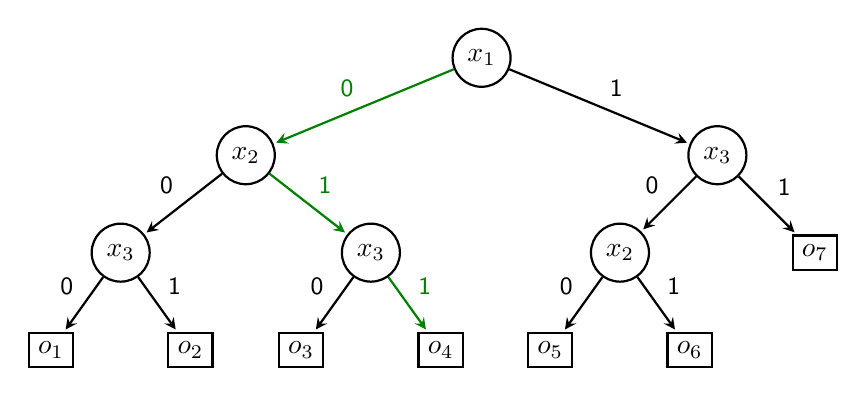
\begin{tikzpicture}[->,>=stealth,shorten >=1pt,auto,node distance=1.75cm, thick,main node/.style={scale=0.9,circle,draw,font=\sffamily\normalsize}]

        \node[circle, draw] (1)[] {$x_1$};

        \node[circle, draw] (2) [below left of=1, xshift=-50, ]{$x_2$};
        \node[circle, draw] (3) [below right of=1, xshift=50, ]{$x_3$};

        \node[circle, draw] (4) [below left of=2, xshift=-10, ]{$x_3$};
        \node[circle, draw] (5) [below right of=2, xshift=10, ]{$x_3$};
        \node[circle, draw] (6) [below left of=3, ]{$x_2$};
        \node[rectangle, draw] (7) [below right of=3]{$o_7$};

        \node[rectangle, draw] (8) [below left of=4, xshift=10]{$o_1$};
        \node[rectangle, draw] (9) [below right of=4, xshift=-10]{$o_2$};
        \node[rectangle, draw] (10) [below left of=5, xshift=10]{$o_3$};
        \node[rectangle, draw] (11) [below right of=5, xshift=-10]{$o_4$};
        \node[rectangle, draw] (12) [below left of=6, xshift=10]{$o_5$};
        \node[rectangle, draw] (13) [below right of=6, xshift=-10]{$o_6$};

        \path[every node/.style={font=\sffamily\small}]
 (1) edge[swap, color=Green]  node{0} (2)
 (1) edge node{1}(3)

 (2) edge[swap]  node{0} (4)
 (2) edge[color=Green]  node{1}(5)

 (3) edge[swap]  node{0} (6)
 (3) edge  node{1}(7)
            
 (4) edge[swap]  node{0} (8)
 (4) edge  node{1}(9)

 (5) edge[swap]  node{0} (10)
 (5) edge[color=Green]  node{1}(11)

 (6) edge[swap]  node{0} (12)
 (6) edge  node{1}(13)
 ;
    \end{tikzpicture}

    \caption{An example of a decision tree of size 13 and depth 3. The green path shows the computation made for the input $x = 011$.}
\end{figure}

Decision trees give an easier way to describe the computation of an oracle Turing machine: if $M^B$ solves (or verifies) a problem $A$ then the $i$-th query made by the procedure corresponds to a variable $x_i$ for the decision tree where $x_i = 1$ if the query returns a positive result and 0 otherwise. In other words, the computation tree of an oracle Turing machine can be viewed as a decision tree.

\begin{proposition}
 Given a search problem $A \in \mathsf{TFNP}$, if there is an oracle Turing machine $M^B$ that solves (or verifies) $A$ then there is a decision tree that solves (or verifies) $A$.
\end{proposition}

The above proposition gives a strong result that allows us to characterize black-box \TFNP through decision trees instead of oracles: \textit{any decision tree separation implies a relativized separation for some oracle} \cite{proofs_circuits_communication, tfnp_characterization}. As in the communication complexity formulation, given a \TFNP problem $R$, we denote with $R^{dt}$ the equivalent $\TFNP^{dt}$ problem, where \textit{dt} stands for \textit{decision tree}. We will omit this notation when the context makes it clear.

\begin{definition}
 We define $\mathsf{FP}^{dt}$ as the set of query search problems $R = (R_n)_{n \in \N}$ for which there exists a polylogarithmic depth decision tree $T_n$ such that $T_n(x) = y$ if and only if $(x,y) \in R_n$. Likewise, we define $\mathsf{FNP}^{dt}$ as the set of query search problems $R = (R_n)_{n \in \N}$ for which there exists a polylogarithmic depth decision tree family $\{T_y\}_{y \in \{0,1\}^m}$ such that $T_y(x) = 1$ if and only if $(x,y) \in R_n$.
\end{definition}

Like protocols, in query search problems the certificate is the verifying decision tree itself. Decision tree reductions are based on a more fine-grained definition, where the function that maps inputs of the first problem to inputs of the second problem is computed by many decision trees with output $\{0,1\}$.

\begin{definition}
 A query search problem $R = (R_m)_{m \in \N}$, where $R_m \subseteq \{0,1\}^m \times O_m$ is said to be many-to-one reducible to a query search problem $S = (S_n)_{n \in \N}$, where $S_n \subseteq \{0,1\}^n \times O_n'$, if for all $m \in \N$ there is an $n \in \N$ for which there is sequence $T = (T_i)_{i \in [n]}$ of decision trees $T_i : \{0,1\}^m \to \{0,1\}$ and a decision tree $T_y^o : \{0,1\}^m \to O_m$ for each $y \in O_n'$ such that:
    \[\forall x \in \{0,1\}^m \;\; (T(x), y) \in S \implies (x, T_y^o(x)) \in R\]
 where $T(x) := (T_1(x), \ldots, T_n(x))$.
\end{definition}

The difference in notation between $T_1, \ldots, T_n$ and $T_y^o$ underlines the fact that the former return a $\{0,1\}$ output, while the latter returns an output in $O_n$. The \textit{size} of the reduction is the number of input bits to $S$, that being $n$. The \textit{depth} $d$ of the reduction is the maximum depth of any tree involved in the reduction, meaning that
\[d = \max (\{\mathrm{depth}(T_i) : i \in [n]\} \cup \{\mathrm{depth}(T_y^o) : o \in O_m\})\]

The complexity of a reduction from $R$ to $S$, written as $S(R)$, is equal to the sum of the log of the size and the minimal depth of a decision tree reduction from $R$ to $S$, that is $S(R) = \log(m) + d$.

\begin{definition}
 Given $S \in \mathsf{TFNP}^{dt}$, we define the class $S^{dt}$ as the subset of \textsf{TFNP}$^{dt}$ problems efficiently reducible through decision trees to the problem $S$, formally $S^{dt} = \{R \in \mathsf{TFNP} \mid S(R) = O(\log^k n)\}$
\end{definition}

\section{Proof Complexity}

Like the white-box model, black-box total search problems can be studied under multiple lenses, such as \textbf{proof complexity}. This branch of complexity theory studies the complexity measures needed for a propositional formula to be proved by propositional proof systems, that being any system of rules that can prove the truthfulness of a propositional formula, i.e. a string made of logical operators applied on a set of $n$ variables, such as $F = x_1 \land (x_1 \to \lnot x_2 \lor x_3)$.

Any statement can be encoded by propositional formulas, which is either a \textit{tautology} (a statement that is always true), a \textit{satisfiable} formula (a statement that can be true or false based on the assignment) or an \textit{unsatisfiable} formula (a statement that is always false). Proving that a formula $F$ is a tautology is equivalent to proving that $\lnot F$ is unsatisfiable.

Proof systems can be viewed as an algorithm that manipulates propositional formulas, producing a new formula. When a formula $G$ is derived by the formula $F$ in the proof system $S$, we write $F \stackrel{S}{\vdash} G$. Proof systems must be \textit{sound}: if $F \stackrel{S}{\vdash} G$ then $G$ is a \textit{logical consequence} of $F$, which means that $F \to G$ is a tautology. In 1979, Cook and Reckhow gave the following formal definition of propositional proof system - often called Cook-Reckhow proof systems.

\begin{definition}
 A propositional proof system (or pps) is a polynomial time computable surjective function $f : \Sigma^* \to \mathrm{TAUT}$, where $\mathrm{TAUT}$ is the set of logical tautologies.
\end{definition}

Given a formula $F \in \mathrm{TAUT}$ a string $s \in \Sigma^*$ and a proof system $f$, we say that $s$ encodes $F$ for the pps $f$ if it holds that $f(s) = F$. This idea justifies why we want proof systems to be surjective: any true statement must have a valid encoding in the proof system. This property is called \textit{completeness} of the proof system.

The most studied proof system is \textbf{Resolution} (or \textsf{Res}). Given a formula $F \in \mathrm{TAUT}$, this proof system can prove that it is a tautology by proving that $\lnot F \in \mathrm{UNSAT}$.

A \textit{conjunctive normal form} (CNF) formula $F$ is a conjunction of $m$ \textit{clauses} $C_1, \ldots, C_m$, where $C_i$ is a disjunction of $k_i$ \textit{literals}, that being either a variable defined on $F$ or its negation. For example, the following formula is in conjunctive normal $F = (x_1 \lor x_2 \lor \lnot{x_3} \lor x_4) \land (x_1 \lor \lnot{x_2}) \land x_3$

Any formula can be expressed as an equivalent CNF formula, making Resolution a \textit{complete} and \textit{sound} proof system. Resolution proofs are based on repeated applications of the following simple rule called the \textit{resolution rule}:
\[\dfrac{C \lor x \qquad D \lor \lnot x}{C \lor D}\]

Given a CNF formula $F = C_1 \land \ldots \land C_m$ and a clause $C$, we have that $F \stackrel{\mathsf{Res}}{\vdash} C$ if there is a sequence of clauses $D_1, \ldots, D_k$ such that $D_k = C$ and each $D_i$ in the sequence is either an \textit{axiom} of $F$ (meaning that $D_i = C_j$ for some $j$) or is obtained by applying the resolution rule on $D_p$ and $D_q$ for some $p,q < i$. Resolution is able to prove that a CNF formula $\lnot F$ is unsatisfiable by deriving the empty clause $\bot$ starting from the axioms of the formula itself. A Resolution proof is often referred to as a \textit{refutation}.

For example, given the following unsatisfiable CNF formula $(y \lor z) \land (y \lor \overline{z}) \land (x \lor \overline{y} \lor z) \land (\overline{x} \lor \overline{y} \lor z) \land \overline{z}$, a Resolution proof is given by:
\[\begin{array}{lcl}
    D_1 :& \overline{z} & \text{Axiom} \\
    D_2 :& \overline{x} \lor \overline{y} \lor z & \text{Axiom} \\
    D_3 :& x \lor \overline{y} \lor z & \text{Axiom} \\
    D_4 :& \overline{x} \lor \overline{y} & \text{Res. on $D_1, D_2$} \\
    D_5 :& x \lor \overline{y} & \text{Res. on $D_1, D_3$} \\
    D_6 :& y \lor z & \text{Axiom} \\
    D_7 :& y \lor \overline{z} & \text{Axiom} \\
    D_8 :& y & \text{Res. on $D_6,D_7$} \\
    D_9 :& \overline{x} & \text{Res. on $D_4, D_8$} \\
    D_{10} :& x & \text{Res. on $D_5, D_8$} \\
    D_{11} :& \bot & \text{Res. on $D_9, D_10$} \\
\end{array}\]
\noindent

The \textit{length} of a resolution refutation is the number of clauses in the refutation, while the \textit{width} is the maximum number of literals that can be found in any of its clauses. For instance, the previous refutation has length 11 and width 3.

To make things easier to read, each refutation can also be graphically represented by connecting clauses with lines. Resolution refutations expressed in this form are also called DAG-like refutations.

\begin{figure}[H]
    \centering
    
        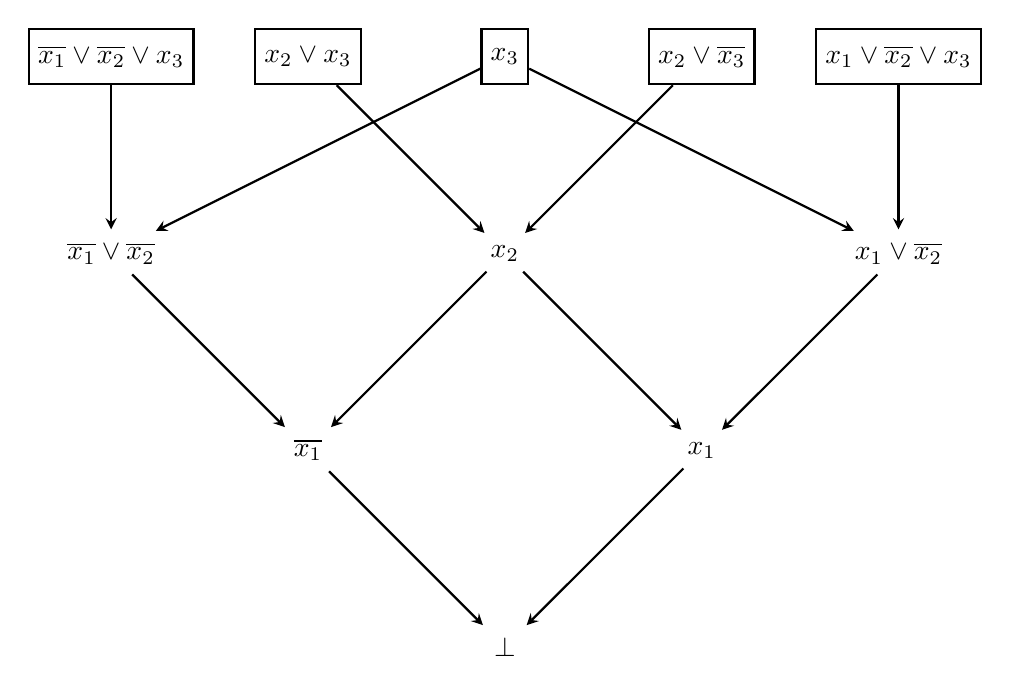
\begin{tikzpicture}[->,>=stealth,shorten >=1pt,auto,node distance=2.5cm, thick,main node/.style={scale=0.9,circle,draw,font=\sffamily\normalsize}]
            \node [rectangle, draw, minimum height=20](1) []{$\overline{x_1} \lor \overline{x_2} \lor x_3$};
            \node [rectangle, draw, minimum height=20](2) [right of=1]{$x_2 \lor x_3$};
            \node [rectangle, draw, minimum height=20](3) [right of=2]{$x_3$};
            \node [rectangle, draw, minimum height=20](4) [right of=3]{$x_2 \lor \overline{x_3}$};
            \node [rectangle, draw, minimum height=20](5) [right of=4]{$x_1 \lor \overline{x_2} \lor x_3$};

            \node (6) [below of=1]{$\overline{x_1} \lor \overline{x_2}$};
            \node (x) [below of=2]{};
            \node (7) [below of=3]{$x_2$};
            \node (y) [below of=4]{};
            \node (8) [below of=5]{$x_1 \lor \overline{x_2}$};

            \node (9) [below of=x]{$\overline{x_1}$};
            \node (10) [below of=y]{$x_1$};
            \node (z) [below of=7]{};
            
            \node (11) [below of=z]{$\bot$};
        
            \path[every node/.style={font=\sffamily\small}]
                (1) edge (6)
                (2) edge (7)
                (3) edge (6)
                (3) edge (8)
                (4) edge (7)
                (5) edge (8)

                (6) edge (9)
                (7) edge (9)
                (7) edge (10)
                (8) edge (10)

                (9) edge (11)
                (10) edge (11)
                ;
        \end{tikzpicture}
    
    \caption{Dag-like refutation of the previous formula.}
\end{figure}

By definition, each clause $D_i$ can be used as premise for more than one rule application, both through weakening and resolution. When each $D_i$ of the proof is used \textbf{only once}, we say that it is a \textbf{tree-like refutation} due to how the underlying DAG becomes a tree. This restriction implies that if we want to use a clause multiple times then it must be derived again (or simply copied if it's an axiom). Clearly, this duplication process allows us to transform any dag-like refutation into a tree-like refutation, but this usually blows up the length of the proof exponentially.

\begin{figure}[H]
    \centering
    
    \resizebox{1\hsize}{!}{
        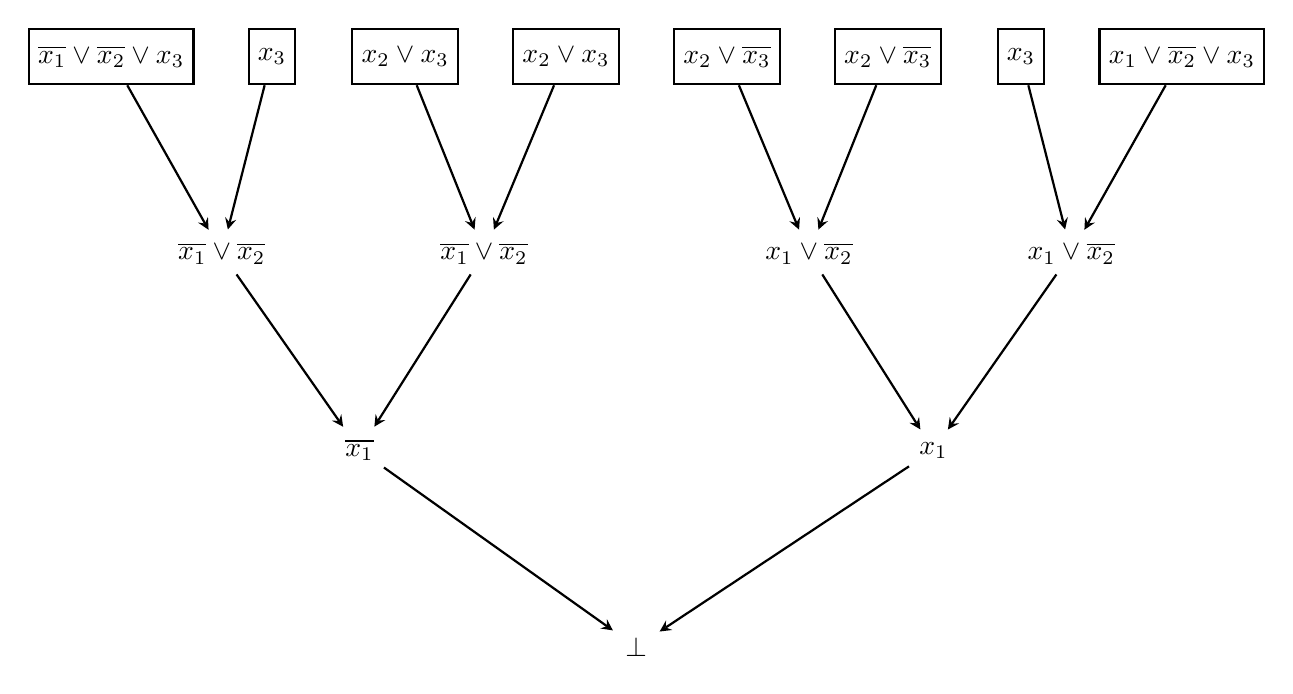
\begin{tikzpicture}[->,>=stealth,shorten >=1pt,auto,node distance=2.5cm, thick,main node/.style={scale=0.9,circle,draw,font=\sffamily\normalsize}]
            \node [rectangle, draw, minimum height=20](1) []{$\overline{x_1} \lor \overline{x_2} \lor x_3$};
            \node [rectangle, draw, minimum height=20](2) [right of=1, xshift=-13]{$x_3$};
            \node [rectangle, draw, minimum height=20](3) [right of=2, xshift=-23]{$x_2 \lor x_3$};
            \node [rectangle, draw, minimum height=20](4) [right of=3, xshift=-13]{$x_2 \lor x_3$};
            \node [rectangle, draw, minimum height=20](5) [right of=4, xshift=-13]{$x_2 \lor \overline{x_3}$};
            \node [rectangle, draw, minimum height=20](6) [right of=5, xshift=-13]{$x_2 \lor \overline{x_3}$};
            \node [rectangle, draw, minimum height=20](7) [right of=6, xshift=-23]{$x_3$};
            \node [rectangle, draw, minimum height=20](8) [right of=7, xshift=-13]{$x_1 \lor \overline{x_2} \lor x_3$}; 

            \node (9)[below of=1, xshift=40]{$\overline{x_1} \lor \overline{x_2}$};
            \node (10)[below of=3, xshift=28.5]{$\overline{x_1} \lor \overline{x_2}$};
            \node (11)[below of=6, xshift=-28.5]{$x_1 \lor \overline{x_2}$};
            \node (12)[below of=8, xshift=-40]{$x_1 \lor \overline{x_2}$};

            \node (13)[below of=10, xshift=-45]{$\overline{x_1}$};
            \node (14)[below of=11, xshift=45]{$x_1$};

            \node (15)[below of=13, xshift=100]{$\bot$};
        
            \path[every node/.style={font=\sffamily\small}]
                (1) edge (9)
                (2) edge (9)
                (3) edge (10)
                (4) edge (10)
                (5) edge (11)
                (6) edge (11)
                (7) edge (12)
                (8) edge (12)

                (9) edge (13)
                (10) edge (13)
                (11) edge (14)
                (12) edge (14)

                (13) edge (15)
                (14) edge (15)
                ;
        \end{tikzpicture}
    }
    
    \caption{Tree-like refutation of the previous formula.}
    \label{treelike_res_proof}
\end{figure}

This subset of proofs defines a more specific proof system called \textit{Tree-like Resolution} (or \textsf{TreeRes}). Generally, this type of refutation produces a proof of exponential length compared to the number of variables defined on the formula itself. Resolution and Tree-like Resolution are separated, meaning that some proofs are easy for the former and hard for the latter, making Resolution a stronger proof system.

Resolution has three main complexity measures: size, depth and width. The \textit{size} of a Resolution proof is the total number of nodes appearing in the proof. The \textit{depth} of a Tree-like Resolution proof is the length of the longest path from an axiom to the empty clause. For example, the proof shown in \Cref{treelike_res_proof} has size 9, depth 3 and width 3. These three complexity measures are highly related. For example, if a Tree-like Resolution proof has depth $d$ the size of such proof is $O(2^{d+1})$ since a $d$-depth tree can have at most $2^{d+1}-1$ nodes.

But why are we interested in proving or refusing propositional formulas? We discussed how the $\mathrm{SAT}$ problem is \textsf{NP}-Complete. This clearly implies that the problem $\overline{SAT}$ is \textsf{coNP}-Complete. This fact can be used to show that $\overline{SAT} \leq_m \mathrm{UNSAT} \leq_m \mathrm{TAUT}$, implying that both $\mathrm{UNSAT}$ and $\mathrm{TAUT}$ are also \textsf{coNP}-Complete. Showing that any of these problems is also in $\mathsf{NP}$ would answer the $\mathsf{NP} \stackrel{?}{=} \mathsf{coNP}$ question.

Proof systems are essential to work on this question: given the encoding $\Pi$ of a proof of $F$ in a proof system, a verifier can follow the rules defined by the proof system to prove that $F$ is indeed a tautology. In this case, $\Pi$ serves as a certificate for $F$ while the pps defines the verifier. We give the following equivalent definition of a propositional proof system.

\begin{definition}
 A propositional proof system (or pps) is a verifier $V$ such that $F \in \mathrm{TAUT}$ if and only if there is a string $\Pi \in \Sigma^*$ such that $V(F,\Pi) = 1$ and that runs in polynomial time with respect to $\abs{F} + \abs{\Pi}$. 
\end{definition}

At first glance, one could think that this definition implies that any complete and sound pps proves that $\mathrm{TAUT} \in \mathsf{NP}$. However, we must also consider the length of such proofs: to be an efficient verifier, the length of the certificates must be polynomially bounded by the length of $F$. In other words, it must hold that $\abs{\Pi} = O(\abs{F}^k)$ for some $k \in \N$. This means that in order to prove that $\mathsf{NP} \neq \mathsf{coNP}$, or equivalently that $\mathrm{TAUT} \in \mathsf{NP}$, we must find a \textbf{polynomially bounded proof system}, a pps that uses only polynomially bounded proofs for all tautologies.

\begin{proposition}
 There is a polynomially bounded proof system if and only if $\mathsf{NP} = \mathsf{coNP}$.
\end{proposition}

We already discussed how researchers believe that $\mathsf{NP} \neq \mathsf{coNP}$ is the expected answer to the conjecture. Proving this statement is no easy task: we would have to prove that there is a particular formula $F$ that strictly requires an exponential length encoding for every discovered and undiscovered proof system.

\newpage

\section{The Black-box model and Proof complexity}

Proof complexity is highly related to other branches of complexity theory, including the study of total search problems. In order to get to this relation between proof complexity and $\mathsf{TFNP}^{dt}$, we have to restrict our focus to CNF formulas. By construction, a CNF formula can be unsatisfiable if and only if for all assignments $\alpha(x_1, \ldots, x_n)$ there is a clause $C_i$ that is false. It's easy to see this fact implies that any CNF formula gives rise to an associated search problem: finding a falsified clause inside the formula (if there is any) for each possible assignment.

\begin{definition}
 Given a CNF $F = C_1 \land \ldots \land C_m$ over $n$ variables, we define $\mathrm{Search}(F)$ as the following search problem: given an input assignment $\alpha(x_1, \ldots, x_n)$, return an index $i$ such that the assignment falsifies $C_i$.
\end{definition}

This problem is usually referred to as the \textbf{false clause search problem}. When $F$ is an unsatisfiable CNF formula, $\mathrm{Search}(F)$ is a total search problem since for any input assignment there will always be an unsatisfied clause. Moreover, the search problem of any unsatisfiable formula can easily be solved (or verified) by a decision tree for any formula $F$: if the assignment $\alpha(x_1 = b_1, \ldots, x_n = b_2)$ falsifies the clause $C_i$, define a path $x_1 = b_1, \ldots, x_n = b_n$ on the decision tree and let $C_i$ be the output of such path. In other words, for all $\lnot F \in \mathrm{TAUT}$ it holds that $\mathrm{Search}(F) \in \mathsf{TFNP}^{dt}$. 

\begin{figure}[H]
    \centering
    
    \begin{tikzpicture}[<-,>=stealth,shorten >=1pt,auto,node distance=2cm, thick,main node/.style={scale=0.9,circle,draw,font=\sffamily\normalsize}]
    
        \node (1)[circle, draw]{$y$};
        
        \node (2) at ($(1)+(-2,-1.75)$) [circle, draw]{$z$};
        \node (3) at ($(1)+(2,-1.75)$) [circle, draw]{$z$};
    
        \node (4) [below left of=2]{};
        \node (5) [below right of=2]{};
    
        \node (6) [below of=3, circle, draw]{$x$};
        
        \node (8) [below left of=6, rectangle, draw]{$x \lor \lnot{y} \lor z$};
        \node (9) [below right of=6, rectangle, draw]{$\lnot{x} \lor \lnot y \lor z$};
    
        \node (11) [right of=9, rectangle, draw]{$\lnot{z}$};
    
        \node (14) at ($(8)+(-2.4,0)$) [rectangle, draw]{$y \lor \lnot{z}$};
        \node (15) [left of=14, rectangle, draw]{$y \lor z$};
    
        \path[every node/.style={font=\sffamily\small}]
 (14) edge [swap] node{1} (2)
 (15) edge node{0} (2)
    
 (8) edge node{0}(6)
 (9) edge node[swap]{1}(6)
    
 (6) edge node{0}(3)
 (11) edge [swap] node{1}(3)
    
 (2) edge node {0} (1)
 (3) edge node [swap] {1} (1)
 ;
    \end{tikzpicture}
    
    \caption{Decision tree for the previous unsatisfiable formula.}
    \end{figure}

Similarly, we can show that any total query search problem $R$ can be associated with the search problem of the formula $F$ that describes the set of decision trees that verify $R$. Consider a decision tree $T$ made of the paths $p_1, \ldots, p_k$, each leading to the leaves $\ell_1, \ldots, \ell_k$. The DNF encoding of $T$, written as $D(T)$, is the disjunction over the conjunction of the literals $\alpha_1, \ldots, \alpha_h$ along each of the accepting paths in $T$. In other words, we have that $D_T = p_1 \lor \ldots \lor p_k$ where each $p_i = \alpha_1 \land \ldots \land \alpha_h \land \ell_i$ is an accepting path of $T$. By De Morgan's theorem, $\lnot{D(T)}$ is a CNF.

\begin{proposition}
    \label{Rdt = Search(F)}
 Given a total query search problem $R \subseteq \{0,1\}^n \times O$, for each $n \in \N$ there exists an unsatisfiable CNF formula $F_n$ defined over $\abs{O}$-many variables such that $R_n = \mathrm{Search}(F_n)$. This formula is called canonical CNF encoding of $R_n$.
\end{proposition}

\begin{proof}
 Since $R = (R_n)_{n \in \N} \in \TFNP^{dt}$, for each $y \in O_n$ there is a $\mathrm{polylog}(n)$-depth decision tree $T_y$ that verifies $R_n$. Consider the CNF $F_n := \bigwedge\limits_{y \in O_n} \lnot{D(T_y)}$. Since $R$ is a total search problem, for each input $x$ there is a valid output, implying that at least one tree $T_y$ will have an accepting path, meaning that $D(T_y)$ with input $x$ accepts and therefore $\lnot{D(T_y)}$ with input $x$ rejects, concluding that $F_n$ is unsatisfiable. Moreover, this formulation also concludes that:
    \[(x,y) \in R_n \iff (x,y) \in \mathrm{Search}(F_n)\]
 and thus that $R_n = \mathrm{Search}(F_n)$.

\end{proof}

This result clearly implies that $(R)_{n \in \N} = (\mathrm{Search}(F_n))_{n \in \N}$, where $F_1, F_2, \ldots$ is a family of CNF formulas, and by extension that black-box \TFNP is exactly the study of the false clause search problem. Like in the communication \TFNP case, the upshot is that it is sufficient to restrict our interests to the study of search problems associated with unsatisfiable CNF formulas.

Furthermore, we also notice that the width of each CNF encoding of a given search problem in \textsf{TFNP}$^{dt}$ corresponds to the maximum depth of the decision trees that solve or verify it.

Through this connection, Göös et al. \cite{adventures_monotone_tfnp} showed that many important proof systems are characterized by an associated $\mathsf{TFNP}^{dt}$ search problem and vice versa. Given a proof system $P$ and an unsatisfiable CNF formula $F$, the \textbf{complexity} required by $P$ to prove $F$ is given by:
\[P(F) := \min\{\log \mathrm{size}(\Pi) + \mathrm{deg}(\Pi) : \Pi \text{ is a $P$-proof of } F\}\]
where $\mathrm{size}(\Pi)$ is the the total number of symbols in $\Pi$ and $\mathrm{deg}(\Pi)$ is the \textit{degree} of $\Pi$ associated to $P$, which varies from proof system to proof system. For example, in Tree-like Resolution the degree is the \textit{depth} of the proof, while in Resolution the degree is the \textit{width} of the proof. This degree measure will be specified for the proof systems analyzed in the following sections.

To make things more readable, we will refer to $\mathrm{Search}(F)$ as $S_F$. Since each $\TFNPdt$ problem is equivalent to $S_F$ for some formula $F$, the complexity parameter defined above can be used to give another \textbf{characterization} of $\TFNPdt$ problems.

\begin{definition}
 We say that a proof system $P$ characterizes a $\TFNPdt$ problem $R$ (and reflexively that $R$ characterizes $P$) if it holds that \[R^{dt} = \{S_F : P(F) = \mathrm{polylog}(n)\}\]
 where $F = (F_i)_{i \in \N}$ is a family of formulas. In a stronger sense, it must hold that $R^{dt}(S_F) = \Theta(P(F))$. 
\end{definition}

Again, this implies that the encoding CNF formulas must have a polylogarithmic width. Most of the \TFNP subclasses discussed in previous sections have been shown to have a characterizing proof system:
\begin{itemize}
    \item $\mathrm{FP}^{dt}(S_F) = \Theta(\mathsf{TreeRes}(F))$ \cite{search_problems_dt_model}
    \item $\mathrm{PLS}^{dt}(S_F) = \Theta(\mathsf{Res}(F))$  \cite{approx_counting}
    \item $\mathrm{PPA}^{dt}(S_F) = \Theta(\F_2\textsf{-NS}(F))$ \cite{adventures_monotone_tfnp}
    \item $\mathrm{PPADS}^{dt}(S_F) = \Theta(\textsf{unary-NS}(F))$ \cite{separations_proof_complexity}
    \item $\mathrm{PPAD}^{dt}(S_F) = \Theta(\textsf{unary-SA}(F))$ \cite{separations_proof_complexity}
    \item $\mathrm{SOPL}^{dt}(S_F) = \Theta(\mathsf{RevRes}(F))$ \cite{separations_proof_complexity}
    \item $\mathrm{CLS}^{dt}(S_F) = \Theta(\mathsf{RevResT}(F))$ \cite{separations_proof_complexity}
\end{itemize}

\begin{figure}[H]
    \centering
    
    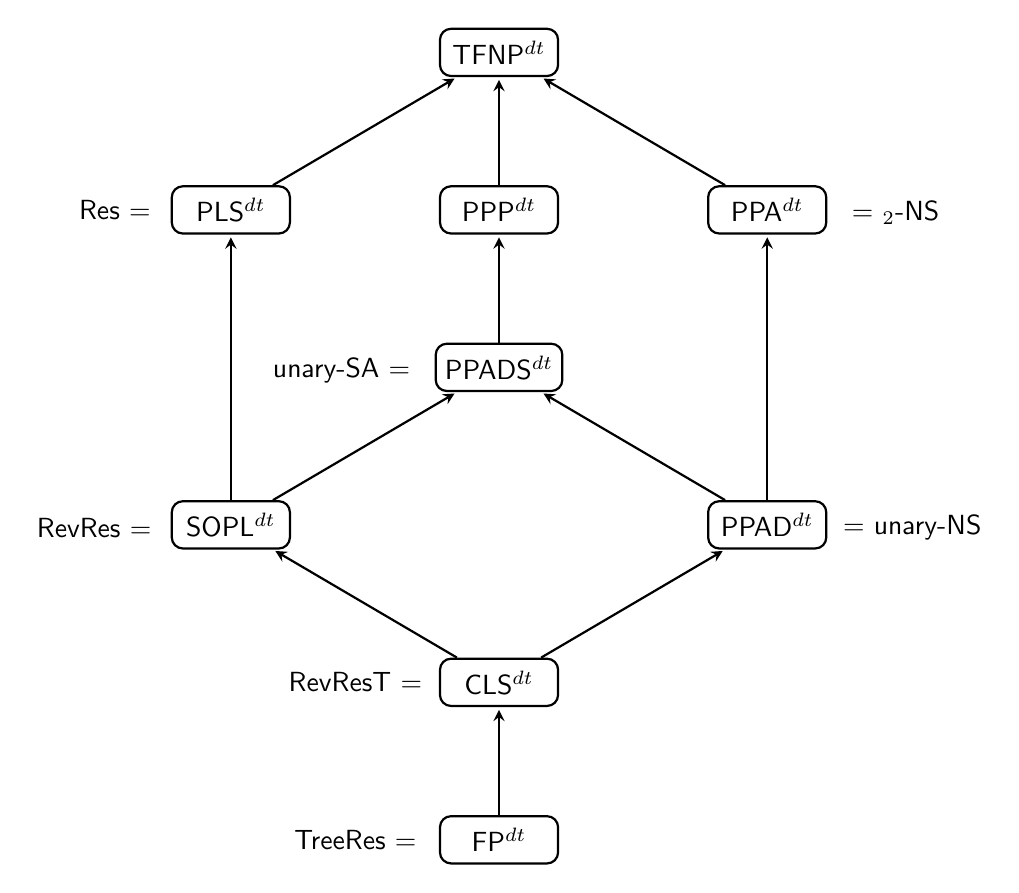
\begin{tikzpicture}[->,>=stealth,shorten >=1pt,auto,node distance=2cm, thick,main node/.style={scale=0.9,circle,draw,font=\sffamily\normalsize}]
    
        \node[rectangle, draw, rounded corners, minimum width=15mm, minimum height=6mm] (2) []{\textsf{TFNP}$^{dt}$};

        \node[rectangle, draw, rounded corners, minimum width=15mm, minimum height=6mm] (3) [below of = 2]{\textsf{PPP}$^{dt}$};

        \node[rectangle, draw, rounded corners, minimum width=15mm, minimum height=6mm] (4) [left of = 3, xshift=-40]{\textsf{PLS}$^{dt}$};

        \node[rectangle, draw, rounded corners, minimum width=15mm, minimum height=6mm] (5) [right of = 3, xshift=40]{\textsf{PPA}$^{dt}$};

        \node[rectangle, draw, rounded corners, minimum width=15mm, minimum height=6mm] (6) [below of = 3]{\textsf{PPADS}$^{dt}$};

        \node (7) [below of = 6]{};

        \node[rectangle, draw, rounded corners, minimum width=15mm, minimum height=6mm] (8) [left of = 7, xshift=-40]{\textsf{SOPL}$^{dt}$};

        \node[rectangle, draw, rounded corners, minimum width=15mm, minimum height=6mm] (9) [right of = 7, xshift=40]{\textsf{PPAD}$^{dt}$};

        \node[rectangle, draw, rounded corners, minimum width=15mm, minimum height=6mm] (10) [below of = 7]{\textsf{CLS}$^{dt}$};

        \node[rectangle, draw, rounded corners, minimum width=15mm, minimum height=6mm] (11) [below of = 10]{\textsf{FP}$^{dt}$};

        \node (12) [left of = 4, xshift = 15]{\textsf{Res} $=$};

        \node (13) [left of = 6, yshift = -1]{\textsf{unary-SA} $=$};
        
        \node (14) [left of = 8, xshift = 7.5, yshift = -1]{\textsf{RevRes} $=$};
        
        \node (15) [left of = 10, xshift = 5]{\textsf{RevResT} $=$};

        \node (16) [right of = 5, xshift = -10.5, yshift = -1]{$=$ \textsf{$\F_2$-NS}};

        \node (17) [right of = 9, xshift = -4.5, yshift = -1]{$=$ \textsf{unary-NS}};

        \node (18) [left of = 11, xshift = 5]{\textsf{TreeRes} $=$};
    
        \path[every node/.style={font=\sffamily\small}]
 (3) edge (2)
 (4) edge (2)
 (5) edge (2)
 (6) edge (3)
 (8) edge (4)
 (8) edge (6)
 (9) edge (5)
 (9) edge (6)
 (10) edge (8)
 (10) edge (9)
 (11) edge (10)
 ;
    \end{tikzpicture}
    
    \caption{Black-box \textsf{TFNP} classes and their characterizing proof systems.}
    \label{TFNP_dt_hierarchy}
\end{figure}

\newpage

\section{Reductions through CNF formulas}

Intuitively, the characterization given in the previous section shows that any $\TFNPdt$ problem can be transformed into a proof system for refuting unsatisfiable CNF formulas of polylogarithmic width: since any $\TFNPdt$ is equivalent to the search problem for some unsatisfiable CNF formula, any efficient decision tree reduction between problems is nothing more than an efficient proof in the characterizing proof system and vice versa. To formalize this idea, we introduce the concept of \textbf{reductions between CNF formulas} \cite{tfnp_characterization}.

Suppose that $C$ is a clause over $n$ variables and that $T = (T_i)_{i \in [n]}$ is a sequence of depth-$d$ decision trees, where $T_i : \{0,1\}^{m} \to \{0,1\}$. We refer to $C(T)$ as the CNF formula obtained by substituting each variable $x_i$ in $C$ with $D(T_i)$ and rewriting the result as a CNF, or more conveniently:
\[C(T) := \bigwedge_{i \in [n]} \, \bigwedge_{\substack{r \,:\, \text{rejecting} \\ \text{path of $T_i$}}} \lnot{r}\]

\begin{definition}
 Let $F = C_1 \land \ldots \land C_{m_F}$ be an unsatisfiable CNF over $n_F$ variables. We say that a CNF formula $H$ made of $m_H$ clauses over $n_H$ variables reduces to $F$ via depth-$d$ decision trees if there exist two sequences of depth-$d$ decision trees $T = (T_i)_{i \in [n_F]}$ and $T^o = (T_j^o)_{j \in [m_F]}$, where $T_i : \{0,1\}^{n_H} \to \{0,1\}$ and $T_j^o : \{0,1\}^{n_H} \to [m_H]$, such that given the following formula:
    \[F_H := \bigwedge_{j \in [m_F]} \,\bigwedge_{\substack{p \,:\; \text{path} \\ \text{in } T_j^o}} C_i(T) \lor \lnot{p}\]
 it holds that if $F$ is unsatisfiable then $F_H$ is unsatisfiable and by consequence that $H$ is unsatisfiable. 
\end{definition}

In particular, we notice that $F_H$ can also be written as a CNF by simply distributing each $\lnot{p}$ inside $C_i(T)$. Each clause $C_i(T) \lor \lnot{p}$ must be either tautological (since it could contain a variable and its negation) or a weakening of the corresponding clause of $H$ - meaning that it is a formula $Q$ such that $H \to Q$ - indexed by the label at the end of the path $p$. Moreover, we notice that through this formulation any depth-$d$ decision tree reduction from $S_H$ to $S_F$ induces the search problem $S_{F_H}$. By construction, reductions between CNF formulas are just a formal way to say that reductions between search problems reduction are actually proof systems.

\begin{definition}
 Given a problem $S_F \in \TFNPdt$ the \textbf{canonical proof system} of such problem, written as $P_F$, is a proof system that refutes an unsatisfiable formula $H$ over $n_H$ variables if $H$ is reducible to an instance of $F$ over $n_F$ variables. 
\end{definition} 

A $P_F$-proof of $H$ consists of the decision trees that make such reduction possible. The \textit{size} of such proof is given by $n_F$, while the \textit{degree} is given by the maximum depth among the involved decision trees. Hence, the $P_F$ complexity of $H$ is given by:
    \[P_F(H) := \min\{\log \mathrm{size(\Pi)}+ \mathrm{depth}(\Pi) : \Pi \text{ is a $P_F$-proof of } H\}\]

This definition directly implies that given $S_F \in \TFNPdt$, the \textbf{characterizing proof system} of $S_F^{dt}$ is equivalent to the canonical proof system $P_F$. Canonical proof systems are \textit{sound}, since by construction any valid substitution of an unsatisfiable CNF formula is also unsatisfiable, and also \textit{efficiently verifiable}, since it suffices to check that each of the clauses of $F_H$ is either tautological or a weakening of a clause in $H$, which can both be done in polynomial time compared to the size of the proof.

The following theorem plays a crucial role in $\TFNPdt$ characterization through proof complexity, stating that the proof system $P_F$ has a short proof of $H$ if and only if $S_H$ efficiently reduces to $S_F$. In other words, an efficient proof of a formula in a characterizing proof system automatically gives an efficient reduction to the corresponding complete search problem.

\begin{theorem}
    \label{equiv_proof}
 Let $S_F \in \TFNPdt$ and let $H$ be an unsatisfiable CNF formula. The two following results hold:
    \begin{enumerate}
        \item If $H$ has a size $s$ and depth $d$ proof in $P_F$ then $S_H$ has a size $O(s)$ and depth $d$ reduction to $S_F$
        \item If $S_H$ has a size $s$ and depth $d$ decision tree reduction to $S_F$ then $H$ has a size $s2^{O(d)}$ and depth $d$ proof in $P_F$
    \end{enumerate}
 In particular, this implies that $S_F^{dt}(S_H) = \Theta(P_F(H))$.
\end{theorem}


\begin{proof}
 Suppose that $T = (T_i)_{i \in [n_F]}$ and $T' = (T_j^o)_{j \in [m_F]}$ is a $P_F$ proof of $H$ of size $s$ and depth $d$. Given any assignment $\alpha$ such that $(\alpha, i) \in S_F$, let $C_i$ be the clause of $F$ falsified by $T_1(\alpha), \ldots, T_{n_F}(\alpha)$ and let $p$ be the path followed by $T_i^o(\alpha)$. It's easy to see that a clause of the formula $C_i(T) \lor \lnot{p}$ must be falsified by $\alpha$. In particular, such clause is also the weakening of the $T_i^o(\alpha)$-th clause of $H$, concluding that $(\alpha, T_i^o(\alpha)) \in S_H$. In other words, the $P_F$ proof of $H$ corresponds to a reduction from $S_H$ to $S_F$ of size $n_F = O(s)$ and depth $d$.

 Vice versa, suppose that $T = (T_i)_{i \in [n_F]}$ and $T' = (T_j^o)_{j \in [m_F]}$ is a decision tree reduction from $S_H$ to $S_F$ of size $s$ and depth $d$. Then, we can construct $F_H$ as previously described through the use of these decision trees. Let $L$ be a clause of $C_i(T)$ for some $i \in [m_F]$ and let $p$ be any path in $T_i^o$. If the formula $C_i(T) \lor \lnot{p}$ is tautological, then it can be ignored since $F_H$ is a CNF. Otherwise, let $\alpha$ be an assignment that falsifies $L \lor \lnot{p}$. Then, it holds that $T_1(\alpha), \ldots, T_{n_F}(\alpha)$ falsifies $C_i(T)$ and that $T_i^o(\alpha)$ follows path $p$. Thus, the $T_i(\alpha)$-th clause of $\lnot{H}$ must also be false, implying that $L \lor \lnot{p}$ is a weakening of such clause. This concludes that $F_H$ is a $P_F$-proof of $H$ of depth at most $d$ (due to how $F_H$ is constructed) and thus that the size is at most $s2^{O(d)}$.

\end{proof}

\cleardoublepage
